\documentclass[12pt]{beamer}

\usepackage[english]{babel}
\usepackage[utf8]{inputenc}
\usepackage{tikz}

\usetheme{Copenhagen}
\setbeamertemplate{navigation symbols}{}

\title{The FLP Theorem}
\author[Jacopo Notarstefano]{
  Jacopo Notarstefano\\
  \texttt{jacopo.notarstefano [at] gmail.com}
}
\date{November 26, 2014}

\begin{document}
  \begin{frame}[plain]
    \titlepage
  \end{frame}

  \begin{frame}{The Distributed Consensus Problem}
    \begin{definition}{}
    \end{definition}
  \end{frame}

  \begin{frame}{Consensus protocol}
    \begin{definition}[Consensus protocol]
      A \textbf{consensus protocol} is an asynchronous system of \(N\) processes (\(N\ge 2\)). Each process \(p\) has a one-bit \textbf{input register} \(x_p\), an \textbf{output register} \(y_p\) with values in \(\{\bot, 0, 1\}\) and an unbounded amount of internal storage.
    \end{definition}

    \vspace{0.25cm}

    \textbf{Initial states} prescribe fixed starting values for all but the input register; in particular, the output register starts with value \(\bot\).

    \vspace{0.25cm}

    \(p\) acts deterministically according to a \textbf{transition} function.
  \end{frame}

  \begin{frame}{Decision states}
    The states in which the output register has value \(0\) or \(1\) are distinguished as being \textbf{decision states}. The transition function cannot change the value of the output register once the process has reached a decision state; that is, the output register is ``write-once''.

    \vspace{0.25cm}

    \begin{figure}
      \makebox[\textwidth][c]{
        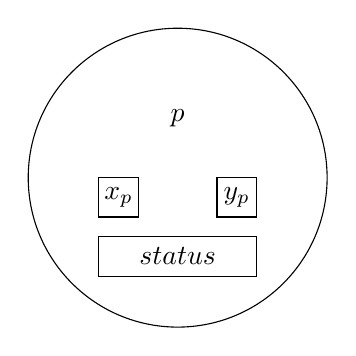
\begin{tikzpicture}
          \tikzstyle{process}=[circle, draw, inner sep=0pt, minimum size=108pt]

          \node (p) at (0, 0) [process] {};
          \node (plabel) at (0, 0.75) [] {\(p\)};
          \node (xp) at (-0.75, -0.25) [] {\(x_p\)};
          \node (yp) at ( 0.75, -0.25) [] {\(y_p\)};
          \node (status) at (0, -1) [] {\(\text{status}\)};

          \draw (-1, -0.5) -- (-1, 0) -- (-0.5, 0) -- (-0.5, -0.5) -- cycle;
          \draw ( 1, -0.5) -- ( 1, 0) -- ( 0.5, 0) -- ( 0.5, -0.5) -- cycle;
	  \draw (-1, -1.25) -- (-1, -0.75) -- (1, -0.75) -- (1, -1.25) -- cycle;
        \end{tikzpicture}
      }
    \end{figure}
  \end{frame}

  \begin{frame}{Message system}
    A \textbf{message} is a pair \((p,m)\), where \(p\) is the name of the destination process and \(m\) is a ``message value'' from a fixed universe \(M\).

    \vspace{0.25cm}

    \begin{definition}[Message system]
      The \textbf{message system} mantains a multiset, called the \textbf{message buffer}, of messages that have been sent but not yet delivered. It supports two abstract operations:
      \begin{description}
        \item[\texttt{ send(p,m)}:] Places \((p,m)\) in the message buffer.
	\item[\texttt{receive(p)}:] Deletes some message \((p,m)\) from the buffer and returns \(m\), in which case we say \((p,m)\) is \textbf{delivered}, or returns the special null marker \(\varnothing\) and leaves the buffer unchanged.
      \end{description}
    \end{definition}
  \end{frame}

  \begin{frame}{Partial correctness}
    A configuration \(C\) has \textbf{decision value} \(v\) if some process \(p\) is in a decision state with \(y_p = v\).

    \vspace{0.25cm}

    \begin{definition}[Partial correctness]
      A consensus protocol is \textbf{partially correct} if:
      \begin{enumerate}
        \item No accessible configuration has more than one decision value.
        \item For each \(v\in \{0,1\}\), some accessible configuration has decision value \(v\).
      \end{enumerate}
    \end{definition}
  \end{frame}

  \begin{frame}{Total correctness in spite of one fault}
    A process \(p\) is \textbf{nonfaulty} in run if it takes infinitely many steps, otherwise it is \textbf{faulty}.

    \vspace{0.25cm}

    A run is \textbf{admissible} if at most one process is faulty and all messages sent to nonfaulty processes are eventually received.

    \vspace{0.25cm}

    A run is \textbf{deciding} if some process reaches a decision state.

    \vspace{0.25cm}

    \begin{definition}[Total correctness in spite of one fault]
      A consensus protocol \(P\) is \textbf{totaly correct in spite of one fault} if it is partially correct and every admissibile run is deciding.
    \end{definition}
  \end{frame}

  \begin{frame}{Main result}
    \begin{theorem}[Fischer, Lynch, Paterson 1985]
      No consensus protocol is totally correct in spite of one fault.
    \end{theorem}

    \vspace{0.25cm}

    A configuration is \textbf{bivalent} if the set of decision values of configurations reachable from it has \(2\) elements. It is instead \textbf{\(0\)-valent} or \textbf{\(1\)-valent} according to the corresponding value.

    \vspace{0.25cm}

    \begin{proof}[Proof (sketch)]
      Given an initial bivalent configuration, we construct an admissible run that at each stage results in another bivalent configuration.
    \end{proof}
  \end{frame}

  \begin{frame}{Lemma 1}
    \begin{lemma}
      Suppose that from some configuration \(C\), the schedules \(\sigma_1\), \(\sigma_2\) lead to configurations \(C_1\), \(C_2\) respectively. If the sets of processes taking steps in \(\sigma_1\) and \(\sigma_2\), respectively, are disjoint, then \(\sigma_2\) can be applied to \(C_1\) and \(\sigma_1\) can be applied to \(C_2\), and both lead to the same configuration \(C_3\).
    \end{lemma}

    \vspace{0.25cm}

    In other words: \textbf{schedules about disjoint processes commute with each other}.
  \end{frame}

  \begin{frame}{Proof of Lemma 1}
    \begin{proof}[Proof (Lemma 1)]
      \begin{figure}
        \makebox[\textwidth][c]{
          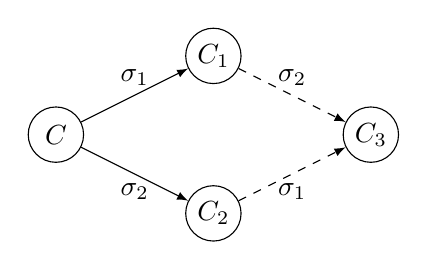
\begin{tikzpicture}
            \tikzstyle{configuration}=[draw,circle,inner sep=0pt,minimum size=20pt]

            \node (C) at (0,0) [configuration] {\(C\)};
            \node (C1) at (2,1) [configuration] {\(C_1\)};
            \node (C2) at (2,-1) [configuration] {\(C_2\)};
            \node (C3) at (4,0) [configuration] {\(C_3\)};

            \draw[-latex] (C) to node[above] {\(\sigma_1\)} (C1);
            \draw[-latex] (C) to node[below] {\(\sigma_2\)} (C2);
            \draw[-latex, dashed] (C1) to node[above] {\(\sigma_2\)} (C3);
            \draw[-latex, dashed] (C2) to node[below] {\(\sigma_1\)} (C3);
          \end{tikzpicture}
        }
      \end{figure}

      Because the sets of processes are disjoint, an event in \(\sigma_1\) applicable to \(C\) is applicable to \(C_2\) as well.

      \vspace{0.25cm}

      Because of determinism, after all events are processed they must end up in the same state.
    \end{proof}
  \end{frame}

  \begin{frame}{Lemma 2}
    \begin{lemma}
      \(P\) has a bivalent initial configuration.
    \end{lemma}

    \vspace{0.25cm}

    \begin{proof}[Proof (Lemma 2)]
    \end{proof}
  \end{frame}

  \begin{frame}{Lemma 3}
    \begin{lemma}
      Let \(C\) be a bivalent configuration of \(P\), and let \(e = (p,m)\) be an event that is applicable to \(C\). Let \(\mathcal{C}\) be the set of configurations reachable from \(C\) without applying \(e\), and let \(\mathcal{D} = e(\mathcal{C}) = \{ e(E) \vert E \in \mathcal{C} \text{ and } e \text{ is applicable to \(E\)} \}\). Then, \(\mathcal{D}\) contains a bivalent configuration.
    \end{lemma}

    \vspace{0.25cm}

    In other words: given a bivalent configuration and an event \(e\) applicable to it, \textbf{we construct another bivalent configuration having \(e\) as the last applied event}.
  \end{frame}

  \begin{frame}{Proof of Lemma 3}
    \begin{proof}[Proof (Lemma 3)]
    \end{proof}
  \end{frame}

  \begin{frame}{Proof of main result}
    \begin{proof}[Proof (main result)]
    \end{proof}
  \end{frame}
\end{document}
